
\documentclass[letterpaper, 10 pt, conference]{ieeeconf}  

\IEEEoverridecommandlockouts                              
\overrideIEEEmargins


\usepackage[utf8]{inputenc}
\usepackage[T1]{fontenc}
\usepackage{wrapfig}
\usepackage{graphicx}
\usepackage{hyperref}


\title{\LARGE \bf
MÉTODO DE MONTE CARLO PARA EL CÁLCULO DE PI
}

\author{Universidad Nacional de Loja
\\
Carrera de Ingeniería en Sistemas
\\
Loja-Ecuador
\\
\textbf{cristian.e.medina@unl.edu.ec}
}

\begin{document}
\maketitle



%%%%%%%%%%%%%%%%%%%%%%%%%%%%%%%%%%%%%%%%%%%%%%%%%%%%%%%%%%%%%%%%%%%%%%%%%%%%%%%%


%%%%%%%%%%%%%%%%%%%%%%%%%%%%%%%%%%%%%%%%%%%%%%%%%%%%%%%%%%%%%%%%%%%%%%%%%%%%%%%%
\section{\textbf{DESARROLLO}}
    El método "Monte Carlo" es una estrategia de resolución de problemas que utiliza estadísticas: si la probabilidad de un determinado evento es P, podemos simular aleatoriamente este evento y obtener P haciendo (número de veces que ocurrió nuestro evento) / (simulaciones totales)\cite{metodomontecarlo}.
    \newline
    \newline
    De esta manera, sabemos que el área del cuadrado en azul es 1 y el área del área roja es pi / 4. Si generamos N números aleatorios dentro del cuadrado, el número de puntos que caen en el círculo M dividido por el número total de números generados N tendrá que aproximarse al área del círculo y, por lo tanto, p / 4.
Básicamente obtendremos pi = 4 * M / N.

 \begin{figure}[!ht]
\centering
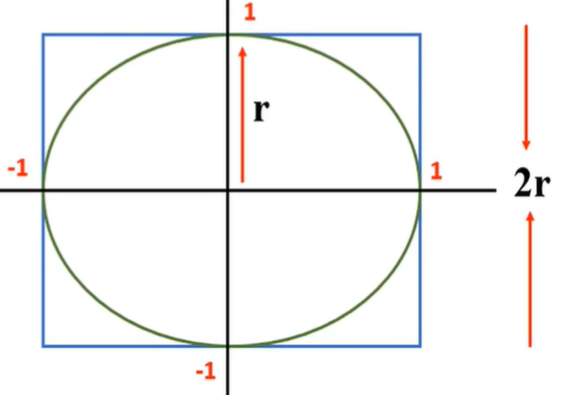
\includegraphics[width=0.3\textwidth]{images/fig1.png}
\caption{Radio de una circunferencia}
\label{fig:estructurados}
\end{figure}
Para deducir la fórmula anterior se sabe que:
\begin{itemize}
    \item El área de una circunferencía es:
     \begin{figure}[!ht]
\centering

\includegraphics[width=0.3\textwidth]{images/ecu1.png}
\label{fig:estructurados}
\end{figure}
\item El área de un cuadrado es:
 \begin{figure}[!ht]
\centering

\includegraphics[width=0.3\textwidth]{images/ecu2.png}
\label{fig:estructurados}
\end{figure}
\item Para el calculo del evento P obtenemos que:
 \begin{figure}[!ht]
\centering

\includegraphics[width=0.3\textwidth]{images/ecu3.png}
\label{fig:estructurados}
\end{figure}
\newline
Una vez obtendo podemos despejar y obtener:
 \begin{figure}[!ht]
\centering

\includegraphics[width=0.3\textwidth]{images/ecu4.png}
\label{fig:estructurados}
\end{figure}
\end{itemize}
Para realizar el cálculo de pi por el método de Monte en Excel definimos un intervalo para nuestro cuadrado en el eje x y en el eje y, esto nos permitirá generar números aleatorios dentro de dicho intervalo.

\begin{figure}[!ht]
\centering
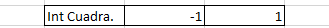
\includegraphics[width=0.4\textwidth]{images/intervalo.png}
\caption{intervalo del cuadrado}
\label{fig:estructurados}
\end{figure}
Para generar números aleatorios a partir del intervalo se utilizó la siguiente formula de Excel:
\begin{figure}[!ht]
\centering
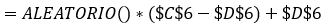
\includegraphics[width=0.4\textwidth]{images/form1.png}
\label{fig:estructurados}
\end{figure}

\begin{figure}[!ht]
\centering
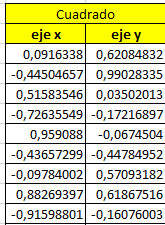
\includegraphics[width=0.3\textwidth]{images/cuad.png}
\caption{Valores aleatorios en el eje x y y del cuadrado }
\label{fig:estructurados}
\end{figure}

En la figura 3 se puede observar un fragmento de la tabla de los valores obtenidos para el eje x y y denotados por la formula de generacion de aleatorios en un intervalo.
\newline
\newline
Para definir el valor de x y y de la circunferencia se utilizó la siguiente formula:

\begin{figure}[!ht]
\centering
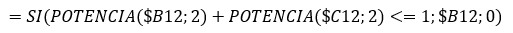
\includegraphics[width=0.4\textwidth]{images/form2.png}
\label{fig:estructurados}
\end{figure}          
Cuya condicional define el área del circulo dentro del cuadrado, la condición establece que si es que los valores aleatorios se encuentran dentro del área del circulo va a ser igual al valor del eje x y y, si no es así este será cero.
\begin{figure}[!ht]
\centering
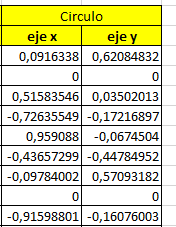
\includegraphics[width=0.3\textwidth]{images/circun.png}
\caption{Valores en el eje x y y de la circunferencia}
\label{fig:estructurados}
\end{figure}
\newline
La representación gráfica de estos valores es:
\begin{figure}[!ht]
\centering
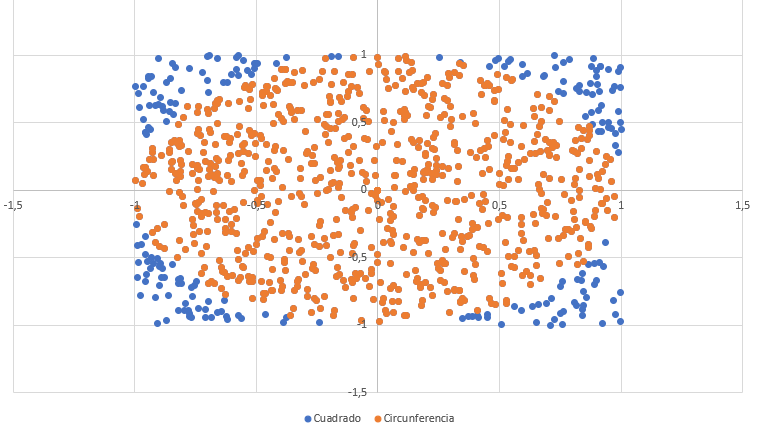
\includegraphics[width=0.5\textwidth]{images/graffinal.png}
\caption{representación gráfica de los valores cuadrado y la circunferencia}
\label{fig:estructurados}
\end{figure}
\newline
Para poder sumar los elementos que se encuentran dentro de la circunferencia primero se utilizó la fórmula:
\begin{figure}[!ht]
\centering
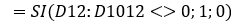
\includegraphics[width=0.3\textwidth]{images/form3.png}
\label{fig:estructurados}
\end{figure}
\newline
La cual establece que si el intervalo en el eje x o y es diferente de cero el resultado será uno caso contrario esta cera cero.
\begin{figure}[!ht]
\centering
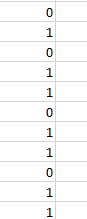
\includegraphics[width=0.1\textwidth]{images/presum.png}
\caption{Valores previos a la suma}
\label{fig:estructurados}
\end{figure}
\newline
Esta tabla residual nos permite contar el número de valores que se encuentran dentro de la circunferencia mediante la fórmula: 
\begin{figure}[!ht]
\centering
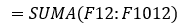
\includegraphics[width=0.3\textwidth]{images/form4.png}
\label{fig:estructurados}
\end{figure}
\newline
También se calcula el numero de valores en número de elementos mediante:
\begin{figure}[!ht]
\centering
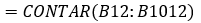
\includegraphics[width=0.3\textwidth]{images/form5.png}
\label{fig:estructurados}
\end{figure}
\newline
Luego se calcula el Área Cir./ Área Cuad.:
\begin{figure}[!ht]
\centering
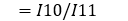
\includegraphics[width=0.3\textwidth]{images/form6.png}
\label{fig:estructurados}
\end{figure}
\newline
Y finalmente para obtener el valor de pi aproximado, en valor de calculado anteriormente se multiplica por cuatro:
\begin{figure}[!ht]
\centering

\includegraphics[width=0.3\textwidth]{images/form7.png}
\label{fig:estructurados}
\end{figure}
\newline
Como resultado final obtenemos la siguiente tabla:
\begin{figure}[!ht]
\centering
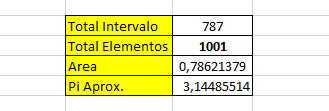
\includegraphics[width=0.4\textwidth]{images/cuadrofinal.png}
\caption{Tabla pi aproximado}
\label{fig:estructurados}
\end{figure}
\newline
\section{\textbf{ANEXOS}}
Hoja de calculo de Exel 
\url{https://1drv.ms/x/s!AucuxkM6z2oboUxuHcaNzrqIAex_}


\bibliographystyle{ieeetr}
\bibliography{cita}
\end{document}
